\documentclass{article}
\usepackage{graphicx} % Required for inserting images
\usepackage{hyperref}
\usepackage{tikz}

\title{Project Submission: An Equivalent to the Written Examination}
\author{
  Darius Fr\u{a}\c{t}il\u{a}\\
  Theodor Moise
}
\date{June 2023}

\begin{document}

\maketitle

\section{Project Overview}
In this project, we aim to develop a robust application that enables users to perform essential CRUD (Create, Read, Update, and Delete) operations on an existing NF3-compliant database. We will utilize the power of C\# and WPF (Windows Presentation Foundation) technology to accomplish this. Additionally, we will leverage the seamless integration between Visual Studio and PostgreSQL to establish a seamless connection between our application and the database.

\vspace{10pt}

\section{Documentation}
\subsection{Related Links}
\begin{itemize}
    \item Microsoft Visual Studio: \href{https://learn.microsoft.com/en-us/visualstudio/get-started/csharp/tutorial-wpf?view=vs-2022}{Used for application development}
    \item EnterpriseDB: \href{https://www.enterprisedb.com/postgres-tutorials/how-connect-postgresql-using-sql-developer-visual-studio-and-dbeaver}{Used for PostgreSQL database connection}
    \item EntityFramework: \href{https://learn.microsoft.com/en-us/visualstudio/data-tools/create-a-simple-data-application-with-wpf-and-entity-framework-6?view=vs-2022}{Used for working with relational databases}
\end{itemize}

\vspace{10pt}

\section{Key Programming Tools Used}
The main programming tools used in the C\# WPF application are:

\vspace{5pt}

\begin{itemize}
    \item Windows Presentation Foundation (WPF): WPF is a framework for developing graphical user interfaces in C\#. It is based on XAML (eXtensible Application Markup Language) and provides a powerful and flexible approach to creating attractive and interactive user interfaces.

    \item Model-View-ViewModel (MVVM): MVVM is a widely used architectural pattern in WPF application development. It clearly separates the presentation logic (View) from the business logic (ViewModel) and data model (Model). MVVM facilitates testing, modularity, and code maintainability.

    \item Data Binding: Data Binding enables direct connection of data from the ViewModel to the user interface elements (View). It ensures automatic synchronization of data between the ViewModel and View and provides an efficient way of handling user interaction with the application.

    \item Styling and Templating: WPF offers a powerful styling and templating system that allows customization of the appearance and behavior of interface elements. This enables the creation of unique and aesthetic graphical interfaces.

    \item Entity Framework (EF): EF is an Object-Relational Mapping (ORM) framework for C\# that simplifies working with relational databases. EF provides a set of tools and abstractions that streamline database interactions and efficiently handle CRUD (Create, Read, Update, Delete) operations.
\end{itemize}

\vspace{10pt}

\section{Entity Relationship Diagram}
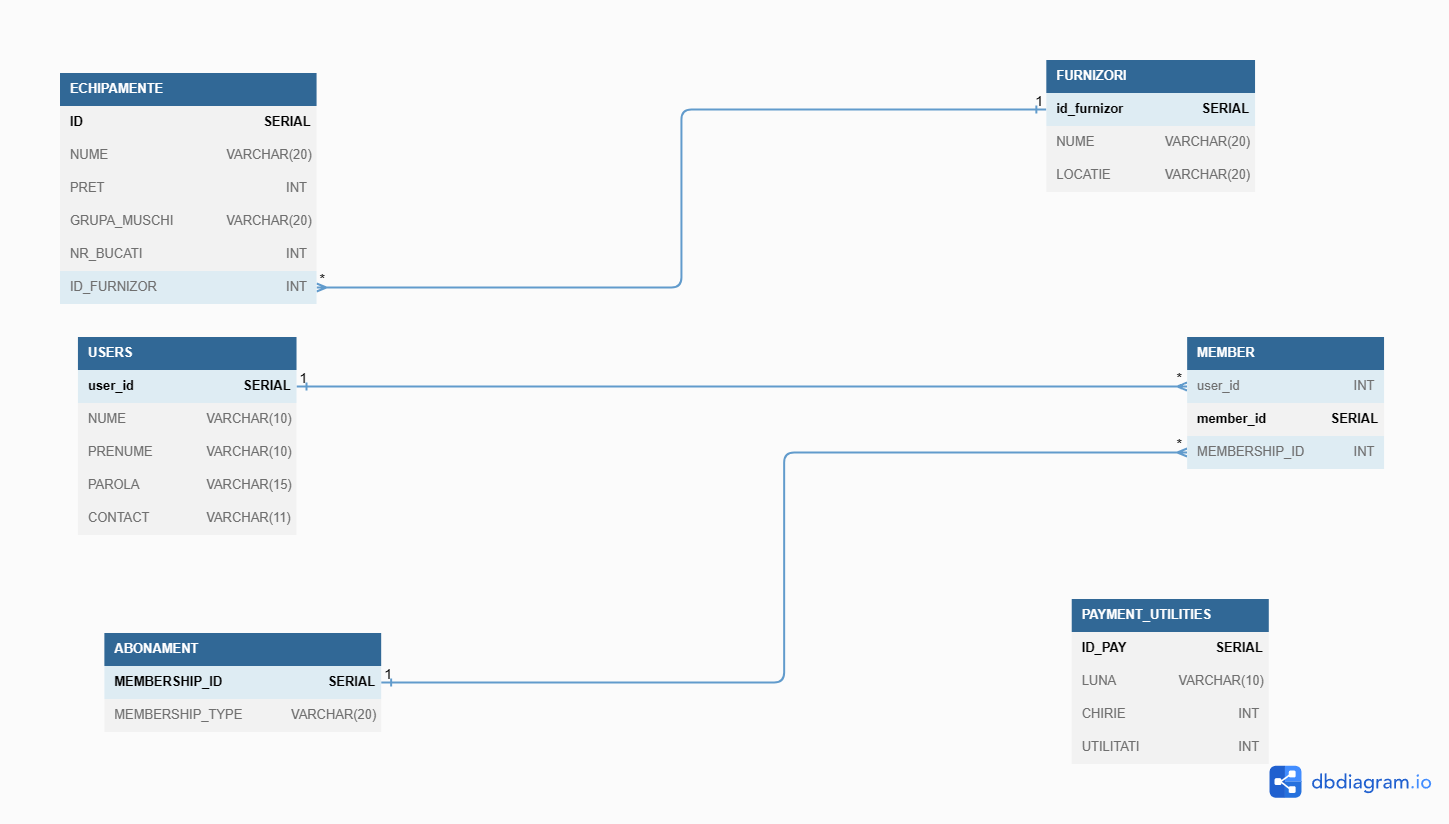
\includegraphics[scale=0.3]{gymeerg.png}

\vspace{10pt}

\section{Project Contributions}
\begin{itemize}
    \item Darius Fr\u{a}\c{t}il\u{a}
    \begin{itemize}
        \item Created the views 
        \item Reconstructed the database
        \item Documentation
    \end{itemize}
    \item Theodor Moise
    \begin{itemize}
        \item Established database connection
        \item Created Postgresql functions
        \item Implemented the viewmodels
    \end{itemize}
\end{itemize}

\end{document}
